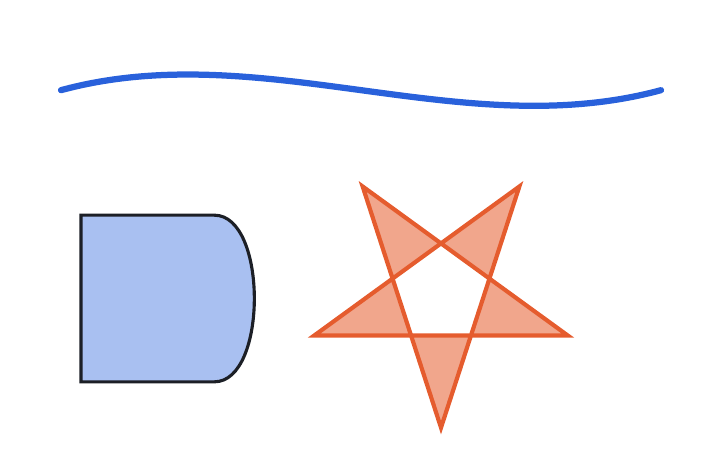
\begin{tikzpicture}[every node/.style={inner sep=0bp,outer sep=0bp}]
  \definecolor{qcA}{rgb}{0.16,0.38,0.86}
  \definecolor{qcB}{rgb}{0.11,0.12,0.15}
  \definecolor{qcC}{rgb}{0.9,0.36,0.18}
  \useasboundingbox (0bp,0bp) rectangle (240bp,150bp);
  \path[fill=qcA,fill opacity=0.4,draw=qcB,line width=1.125bp] (19.2bp,22.5bp) -- (67.2bp,22.5bp) .. controls (86.4bp,22.5bp) and (86.4bp,82.5bp) .. (67.2bp,82.5bp) -- (19.2bp,82.5bp) -- cycle;
  \path[fill=qcC,fill opacity=0.55,draw=qcC,line width=1.5bp,even odd rule] (148.8bp,6bp) -- (177.014bp,92.833bp) -- (103.149bp,39.167bp) -- (194.451bp,39.167bp) -- (120.586bp,92.833bp) -- cycle;
  \path[draw=qcA,line width=2.25bp,line cap=round,line join=round] (12bp,127.5bp) .. controls (84bp,147bp) and (156bp,108bp) .. (228bp,127.5bp);
\end{tikzpicture}
